% ==============================================================================
% =================================== Aufgabe 4 =================================
% ==============================================================================

\chapter{Aufgabe}
\label{chap:4 Aufgabe}
\thispagestyle{fancy}
\section*{Sie sind der Projektleiter für die Stammdatenbereinigung und -aktualisierung zwischen dem \acs{ERP}-, Buchhaltungs- und \acs{CRM}-Programm im Unternehmen. Für ein und denselben Kunden gibt es mehrere Datensätze: \newline\raisebox{-\totalheight}{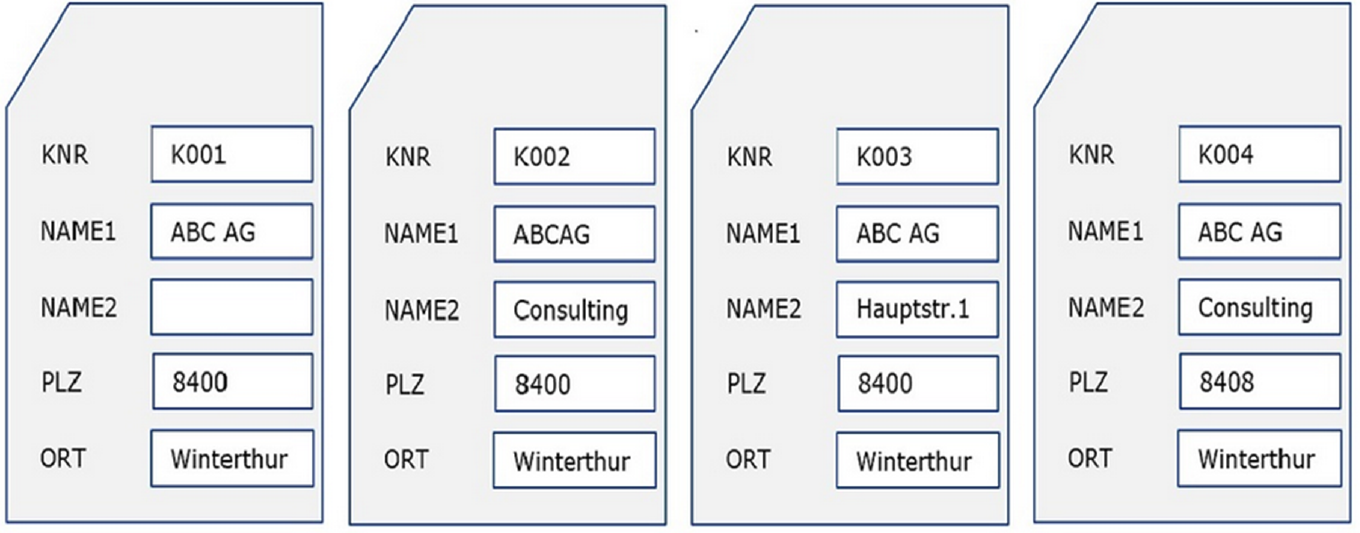
\includegraphics[width=0.95\textwidth]{./asset/image/Stammdaten.png}}\newline\newline Wie können Sie konzeptionell die Stammdaten zentralisieren und aktualisieren?} \par Um die Stammdaten zwischen \acs{ERP}-, Buchhaltungs- und \acs{CRM}-Systemen zu zentralisieren und zu aktualisieren, ist die Implementierung eines \uline{(\textit{\acs{MDM}})-Konzepts} erforderlich. \cite{90} Ziel ist die Schaffung eines \uline{„Single Point of Truth“}, um systemübergreifende Konsistenz und Integrität zu gewährleisten. \cite{90}\cite{91} \par Der konzeptionelle Ansatz gliedert sich in folgende Phasen:
\begin{enumerate}[label=\arabic*.), leftmargin=*]
    \item \textbf{Datenanalyse und Bestandsaufnahme (\textit{Data Profiling})} \par Zunächst müssen die vorhandenen Datensätze aus allen drei Quellsystemen (\textit{\acs{ERP}, \acs{CRM}, Buchhaltung}) technisch analysiert werden. \cite{92}\cite{93}
    \begin{itemize}
        \item \textbf{Identifikation von Duplikaten:} Mittels automatisierter Verfahren werden Übereinstimmungen bei Schlüsselattributen (\textit{\acs{z. B.} Name, Adresse, Geburtsdatum}) gesucht. \cite{94}\cite{95}
        \item \textbf{Qualitätsprüfung:} Es wird ermittelt, welche Felder (\textit{\acs{z. B.} E-Mail, Telefonnummer}) unvollständig oder formal falsch sind. \cite{96}\cite{97}
    \end{itemize}
    \item \textbf{Harmonisierung und Standardisierung} \par Bevor Daten zusammengeführt werden können, müssen sie in ein einheitliches Format gebracht werden. \cite{98}
    \begin{itemize}
        \item \textbf{Strukturierung:} Adressdaten und Telefonnummern werden nach einem festen Schema (\textit{\acs{z. B.} internationale Vorwahlschreibweise}) formatiert. \cite{98}
        \item \textbf{Normierung:} Für Attribute wie „Anrede“ oder „Rechtsform“ werden normierte Wertelisten definiert, um unterschiedliche Schreibweisen (\textit{\acs{z. B.} „GmbH“ \acs{vs.} „Ges. m. b. H.“}) zu eliminieren. \cite{99}
    \end{itemize}
    \item \textbf{Stammdatenbereinigung (\textit{Cleansing und Merging})} \par Bevor Daten zusammengeführt werden können, müssen sie in ein einheitliches Format gebracht werden.
    \begin{itemize}
        \item \textbf{Match \& Merge:} Basierend auf definierten Regeln werden Dubletten zu einem „Golden Record“ (\textit{dem Stammdatensatz mit der höchsten Güte}) zusammengeführt. \cite{100}\cite{101}
        \item \textbf{Festlegung des führenden Systems:} Es muss entschieden werden, welches System für welche Informationen die Hoheit hat. \cite{102} Beispielsweise könnte das CRM für Marketingdaten und die Buchhaltung für zahlungsrelevante Informationen (\textit{Bankverbindung}) federführend sein. \cite{103}\cite{104}
    \end{itemize}
    \item \textbf{Wahl der Zentralisierungs-Architektur} \par Konzeptionell stehen für die dauerhafte Zentralisierung drei Varianten zur Verfügung: \cite{101}
    \begin{itemize}
        \item \textbf{Transaction Hub:} Alle Stammdaten werden ausschließlich in einer zentralen \acs{MDM}-Datenbank gepflegt. \acs{ERP}, \acs{CRM} und Buchhaltung greifen über Services darauf zu. \cite{101}
        \item \textbf{Koexistenz:} Die Daten werden weiterhin in den Systemen gepflegt, aber zeitversetzt mit einer zentralen Master Data Base synchronisiert. \cite{101}
        \item \textbf{Registry:} Die Daten bleiben dezentral, das \acs{MDM}-System verwaltet lediglich Referenzen und erstellt bei Bedarf eine virtuelle Gesamtsicht. \cite{101}
    \end{itemize}
    \item \textbf{Etablierung einer Data Governance} \par Um eine erneute Datenkorruption zu verhindern, müssen Verantwortlichkeiten festgelegt werden:
    \begin{itemize}
        \item \textbf{Data Stewards:} Für die Domäne „Kunde“ wird eine verantwortliche Person oder Abteilung (\textit{\acs{z. B.} Vertriebsinnendienst}) benannt, die jede Neuanlage oder Änderung prüft. \cite{105}
        \item \textbf{Einführung von Workflows:} Änderungen an Stammdaten sollten durch automatisierte Freigabeprozesse (\textit{Änderungsdienst}) dokumentiert werden. \cite{106}
    \end{itemize}
\end{enumerate}
Durch diesen Prozess wird sichergestellt, dass beispielsweise eine Adressänderung im \acs{CRM} automatisch auch in der Buchhaltung und im \acs{ERP}-System aktualisiert wird, wodurch manuelle Mehrfacheingaben und Inkonsistenzen entfallen. \cite{107}\cite{108}

% ==============================================================================
% =================================== Aufgabe 4 =================================
% ==============================================================================